\documentclass[aspectratio=169]{beamer}

\usepackage[utf8]{inputenc}
\usetheme{Madrid}
\usecolortheme{seahorse}

\title{Fase A: Visi Arsitektur dalam Metode Pengembangan Arsitektur TOGAF}
\author{Alfa Yohannis}
\date{\today}

\begin{document}
	
	\frame{\titlepage}
	
	\begin{frame}
		\frametitle{Tujuan}
		\begin{enumerate}			
			\item Mengembangkan visi aspirasional (high-level) mengenai kemampuan dan nilai bisnis yang akan disampaikan sebagai hasil dari arsitektur perusahaan yang diusulkan.
			\item Memperoleh persetujuan untuk Pernyataan Kerja Arsitektur yang mendefinisikan program kerja untuk mengembangkan dan menerapkan arsitektur yang diuraikan dalam Visi Arsitektur.
		\end{enumerate}
	\end{frame}
	
	\begin{frame}
		\frametitle{Input}
		\begin{enumerate}
			\item Permintaan untuk Pekerjaan Arsitektur
			\item Prinsip-prinsip bisnis, tujuan bisnis, dan pendorong bisnis
			\item Model Organisasi untuk Arsitektur Perusahaan
			\item Kerangka Arsitektur yang Disesuaikan, termasuk prinsip-prinsip arsitektur
			\item Repositori Arsitektur yang Terisi; yaitu, dokumentasi arsitektur yang ada (deskripsi kerangka kerja, deskripsi arsitektur, deskripsi dasar yang ada, dll.)
		\end{enumerate}
	\end{frame}
	
	\begin{frame}
		\frametitle{Langkah-langkah}
		\begin{enumerate}
			\item \textbf{Membuat proyek arsitektur}
			\item \textbf{Mengidentifikasi pemangku kepentingan, kekhawatiran, dan persyaratan bisnis}
			\item Mengonfirmasi dan \textbf{mengembangkan} tujuan bisnis, pendorong bisnis, dan batasan
			\item Mengevaluasi kemampuan bisnis
			\item Menilai kesiapan untuk transformasi bisnis
			\item Mendefinisikan ruang lingkup
			\item Mengonfirmasi dan \textbf{mengembangkan} prinsip-prinsip arsitektur, termasuk prinsip-prinsip bisnis
			\item \textbf{Mengembangkan Visi Arsitektur}
			\item \textbf{Mendefinisikan nilai Arsitektur Target yang diajukan dan juga KPInya.} 
			\item \textbf{Mengidentifikasi risiko transformasi bisnis dan aktivitas mitigasi}
			\item \textbf{Mengembangkan} Pernyataan Kerja Arsitektur; \textbf{mendapatkan persetujuan}
		\end{enumerate}
	\end{frame}
	
	\begin{frame}
		\frametitle{Output (1)}
		\begin{enumerate}
			\item Pernyataan Kerja Arsitektur
			\item Pernyataan yang Diperinci tentang Prinsip-prinsip Bisnis, Tujuan Bisnis, dan Pendorong Bisnis
			\item Prinsip-prinsip Arsitektur
			\item Evaluasi Kemampuan
			\item Kerangka Kerja Arsitektur yang Disesuaikan
			\item Visi Arsitektur, termasuk:
			\begin{enumerate}
				\item Deskripsi Masalah
				\item Tujuan Pernyataan Kerja Arsitektur
				\item Tinjauan Ringkasan
				\item Skenario Bisnis (opsional)
				\item Persyaratan Pemangku Kepentingan high-level yang Diperinci
			\end{enumerate}
		\end{enumerate}
	\end{frame}
	
	\begin{frame}
		\frametitle{Output (2)}
		\begin{enumerate}
			\setcounter{enumi}{6}
			\item Draf Dokumen Definisi Arsitektur, termasuk:
			\begin{enumerate}
				\item Arsitektur Bisnis Saat Ini (high-level)
				\item Arsitektur Data Saat Ini (high-level)
				\item Arsitektur Aplikasi Saat Ini (high-level)
				\item Arsitektur Teknologi Saat Ini (high-level)
				\item Arsitektur Bisnis Target (high-level)
				\item Arsitektur Data Target (high-level)
				\item Arsitektur Aplikasi Target (high-level)
				\item Arsitektur Teknologi Target (high-level)
			\end{enumerate}
			\item Rencana Komunikasi
			\item Konten Tambahan yang Melengkapi Repositori Arsitektur
		\end{enumerate}
	\end{frame}
	
	{
		\setbeamertemplate{navigation symbols}{}
		\setbeamertemplate{footline}{}		
		\begin{frame}
			\frametitle{Sample Stakeholders,Stakeholder Analysis, Power vs Interest}
			\begin{columns}
				\begin{column}{0.5\textwidth}
					\begin{center}
						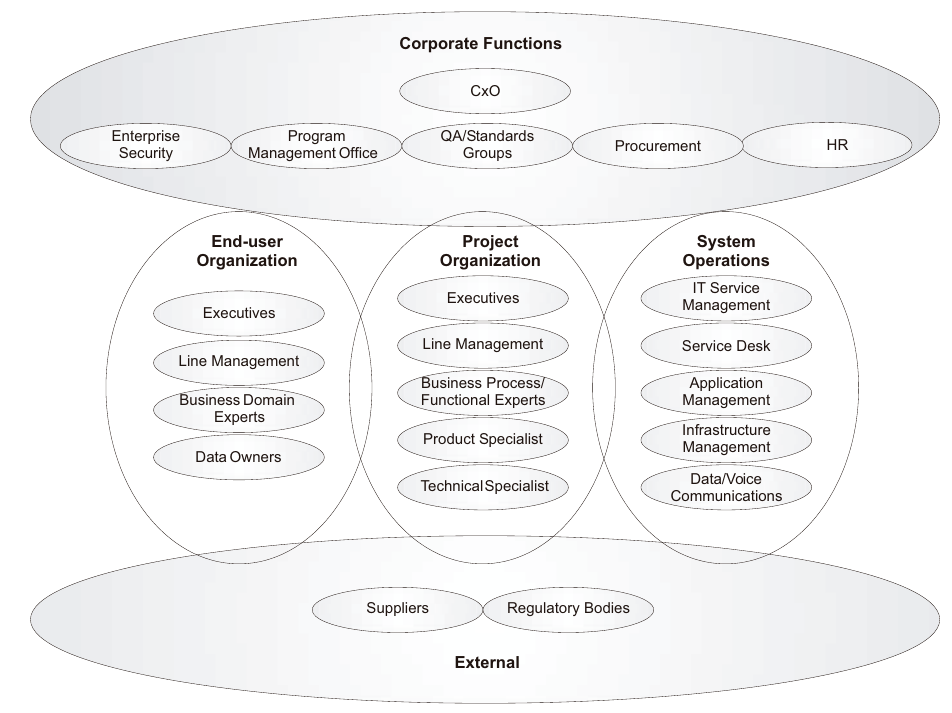
\includegraphics[width=\textwidth]{../figures/sample_stakeholders}
					\end{center}
				\end{column}
				\begin{column}{0.5\textwidth}
					\begin{center}
						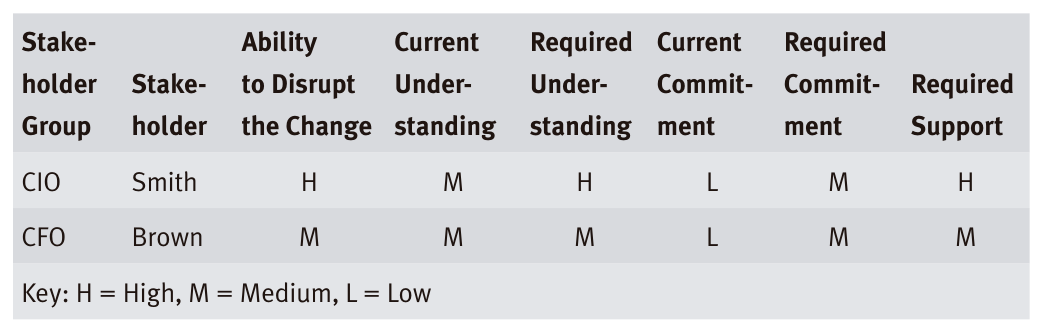
\includegraphics[width=\textwidth]{../figures/stakeholder_analysis}
					\end{center}
					\begin{center}
						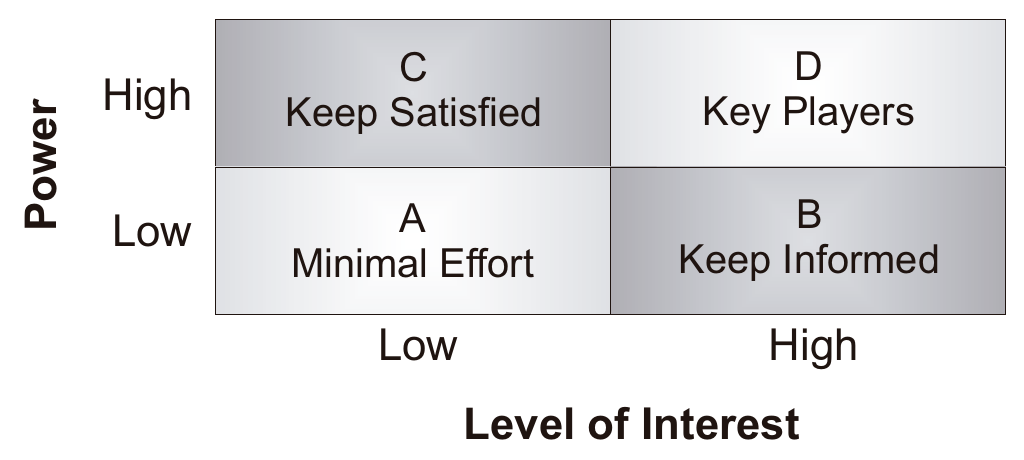
\includegraphics[width=\textwidth]{../figures/power_vs_interest}
					\end{center}
				\end{column}
			\end{columns}
			
		\end{frame}
	}
	
	{
		\setbeamertemplate{navigation symbols}{}
		\setbeamertemplate{footline}{}		
		\begin{frame}
			\frametitle{Stakeholder Map}
			\begin{columns}
				\begin{column}{0.5\textwidth}
					\begin{center}
						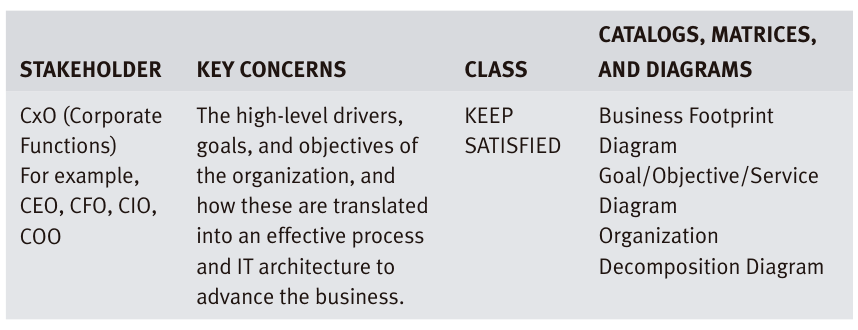
\includegraphics[width=\textwidth]{../figures/stakeholder_map_1}
						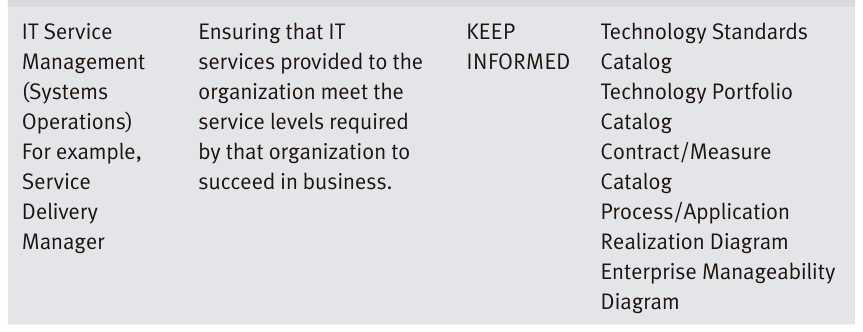
\includegraphics[width=\textwidth]{../figures/stakeholder_map_3}
					\end{center}
					
				\end{column}
				\begin{column}{0.5\textwidth}
					\begin{center}
						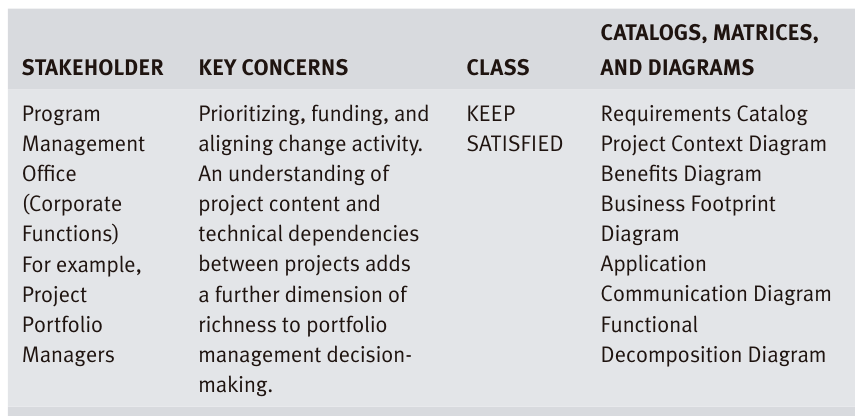
\includegraphics[width=\textwidth]{../figures/stakeholder_map_2}
					\end{center}
				\end{column}
			\end{columns}
			
		\end{frame}
	}
	
	\begin{frame}
		\frametitle{Menilai Kesiapan untuk Transformasi}
		\begin{columns}
			\begin{column}{0.5\textwidth}
				\begin{enumerate}
					\item Visi
					\item Keinginan atau kesediaan untuk mencapai hasil
					\item Kebutuhan
					\item Ada indikasi/kasus di bisnis
					\item Dana
					\item Sponsorship dan kepemimpinan
					\item Tata kelola
					
				\end{enumerate}
			\end{column}
			\begin{column}{0.5\textwidth}
				\begin{enumerate}
					\setcounter{enumi}{7}
					\item Accountabilty (kemampuan untuk dipertanggungjawabkan)
					\item Pendekatan dan model eksekusi yang dapat dikerjakan
					\item Kapasitas TI untuk mengkesekusi
					\item Kapasitas perusahaan untuk mengeksekusi
					\item Kemampuan perusahaan untuk menerapakan dan mengoperasikan pasca eksekusi
				\end{enumerate}
			\end{column}
		\end{columns}
	\end{frame}
	
	\begin{frame}
		\frametitle{Visi Arsitektur}
		\begin{enumerate}
			\item Deskripsi masalah, termasuk para pemangku kepentingan dan kekhawatiran mereka, serta daftar masalah/skenario yang perlu ditangani.
			\item Tujuan Pernyataan Kerja Arsitektur.
			\item Ringkasan pandangan yang diperlukan untuk Permintaan Pekerjaan Arsitektur dan Arsitektur Bisnis, Aplikasi, Data, dan Teknologi tingkat tinggi.
			\item Scenario bisnis.
			\item Kebutuhan stakeholder yang sudah dipetakan dan didetilkan.
		\end{enumerate}
	\end{frame}
	

		\begin{frame}
			\frametitle{Skenario Bisnis}
			\begin{enumerate}
				\item \textbf{Masalah}.
				Identifikasi, dokumentasikan, dan rangking masalah yang mendorong proyek.
				\item \textbf{Lingkungan Bisnis dan Teknis}.
				Dokumentasikan sebagai model arsitektur tingkat tinggi, lingkungan bisnis dan teknis di mana situasi masalah terjadi.
				\item \textbf{Tujuan dan Ukuran Keberhasilan}.
				Identifikasi dan dokumentasikan tujuan yang diinginkan, hasil dari penanganan masalah dengan sukses.
				\item \textbf{Pelaku Manusia}.
				Identifikasi pelaku manusia dan tempat mereka dalam model bisnis, partisipan manusia, dan peran mereka.
				\item \textbf{Pelaku Komputer}.
				Identifikasi pelaku komputer dan tempat mereka dalam model teknologi, elemen komputasi, dan peran mereka.
				\item \textbf{Peran dan Tanggung Jawab}.
				Identifikasi dan dokumentasikan peran, tanggung jawab, dan ukuran keberhasilan per pelaku, skrip yang diperlukan per pelaku, dan hasil yang diinginkan dari penanganan situasi dengan benar.
				\item \textbf{Revisi}.
				Periksa kesesuaian tujuan untuk menginspirasi pekerjaan arsitektur berikutnya, dan perbaiki hanya jika diperlukan.
			\end{enumerate}
		\end{frame}
	
		\begin{frame}
			\frametitle{Dokumen Pernyataan Kerja Arsitektur}
			\begin{enumerate}
				\item Judul
				\item Permintaan dan Latar Belakang Proyek Arsitektur
				\item Deskripsi dan Ruang Lingkup Proyek Arsitektur
				\item Tinjauan Visi Arsitektur
				\item Prosedur Perubahan Ruang Lingkup Tertentu
				\item Peran, Tanggung Jawab, dan Deliverables
				\item Kriteria Penerimaan dan Prosedur
				\item Rencana dan Jadwal Proyek Arsitektur
				\item Persetujuan
			\end{enumerate}
		\end{frame}
	
	\begin{frame}
		\frametitle{Ringkasan}
		Fase Visi Arsitektur merupakan langkah awal dalam Metode Pengembangan Arsitektur TOGAF, dimana kita menetapkan ruang lingkup, mengidentifikasi stakeholder, dan mendefinisikan visi arsitektur high-level. Fase ini sangat penting untuk memastikan bahwa proyek arsitektur memiliki dukungan dan arah yang tepat dari awal.
	\end{frame}
	
\end{document}
